\section{Modello Ottimale}
Analizzando i risultati di tutte le sperimentazioni, possiamo evincere che YOLOv8 è il modello che ottiene il maggior incremento nelle prestazioni a seguito della data augmentation effettuata sul dataset termico. Fino a questo punto, abbiamo addestrato la versione "Nano" del modello; quindi per avere una visione più completa delle potenzialità di YOLOv8, ho deciso di addestrare la versione "Large" del modello (\textbf{yolov8l}\cite{27}) su \texttt{augmented-data-2}, mantenendo le 100 epochs. Seguono i risultati ottenuti dal test:

\begin{figure}[ht]
    \centering
    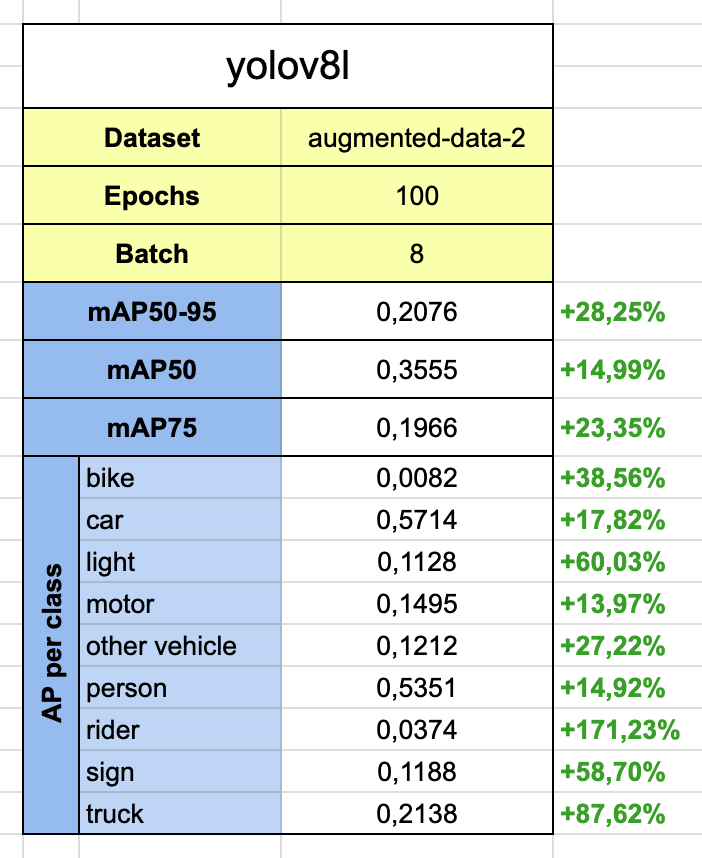
\includegraphics[width=0.5\textwidth]{files/capitoli/4-sperimentazione-risultati/assets/yolov8l-metrics.png}
    \caption{\label{fig:yolov8l-metrics}Risultati test di yolov8l addestrato per 100 epochs sul secondo dataset aumentato a confronto con le metriche ottenute da yolov8n con lo stesso addestramento}
\end{figure}

Notiamo che, a parità di addestramento, con la versione "Large" del modello riusciamo ad ottenere un ulteriore incremento di tutte le metriche rispetto a quelle ottenute dalla "Nano".

\clearpage

\begin{figure}[ht]
    \centering
    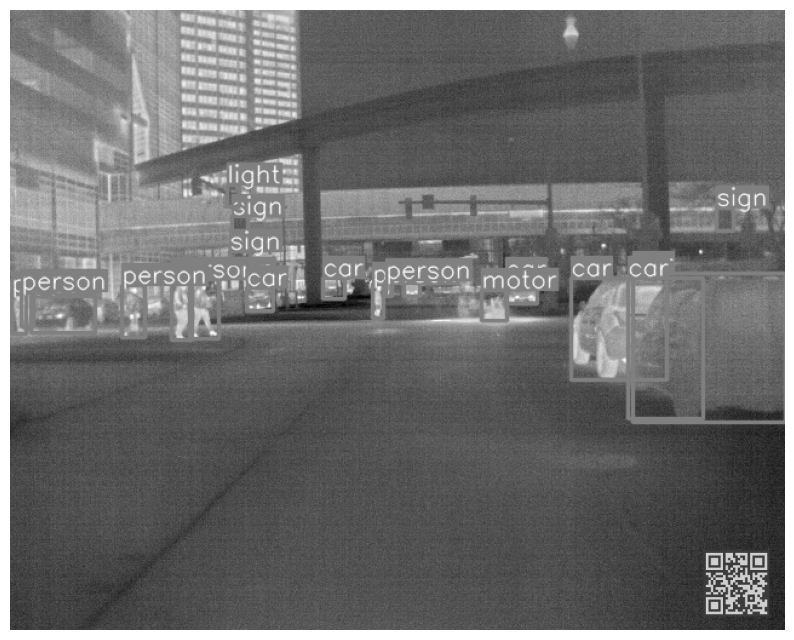
\includegraphics[width=1\textwidth]{files/capitoli/4-sperimentazione-risultati/assets/yolov8l-detections-special.png}
    \caption{\label{fig:yolov8l-detections}Detections effettutate da yolov8l addestrato per 100 epochs sul secondo dataset aumentato}
\end{figure}

\clearpage